\documentclass[a4paper, 12pt]{article}
\usepackage[margin=0.8in]{geometry}
\usepackage{tikz}
\usepackage{scrextend}
\usetikzlibrary{automata,positioning}
\usepackage{graphicx}
\usepackage{pgfplots}
\usepackage{listings}
\usepackage{color}
\usepackage{subcaption}

\definecolor{comments}{rgb}{0,0.5,0.5}
\definecolor{typeWord}{rgb}{0.5,0,1}
\definecolor{number}{rgb}{1,0.5,0}
\definecolor{string}{rgb}{0.5,0.5,0.5}

\lstset{frame=tb,
  language=Java,
  aboveskip=3mm,
  belowskip=3mm,
  showstringspaces=false,
  columns=flexible,
  basicstyle={\small\ttfamily},
  numbers=none,
  numberstyle=\color{number},
  commentstyle=\color{comments},
  stringstyle=\color{string},
  keywordstyle=\color{typeWord},
  breaklines=true,
  breakatwhitespace=true,
  tabsize=4
}

\title{Scotland Yard AI}
\author{Julian Loscombe and Ben Milne}

\begin{document}
\maketitle
\section{Game Tree}
We have set up our game tree to use paralellised Alpha - Beta pruning in order to increase the depth that we can search to in the allotted time. In addition we are using an iterative depth search continually running the tree and updating the best move on each iteration. When the time limit is near we simply grab the last fully computed result.
\subsection{Scoring}
To score our game state we use three main sources of information, the ratio between the PageRank of the detectives' locations and Mr X's location, the ratio between the value of the detectives and MrX's tickets, and the average distance between the detectives and Mr X (using Dijkstra's Algorithm). We consider the average distance to be the most important factor and as such its influence is weighted much higher than the other two. Because it is particularly important to avoid very small distances we use a root function to transform the distance score so that is is much steeper when Mr X is close to being caught. We then normalise the ratios around 0 and apply them to the distance score as below:
\begin{lstlisting}
double score = (10 * Math.pow(detDistance, 0.5));
        score += ((ticketRatio - 1) * kTicketInfluence) * score;
        score += ((pageRankRatio - 1) * kPageRankInfluence) * score;
\end{lstlisting}
This ensures that the average ratio will have no effect on the score and that when the distance is very small it's main objective is to increase that distance. We also added a special case to boost secret move scores when the distance was very small. The below graph illustrates part of the score function.

\begin{figure}[!h]
\centering
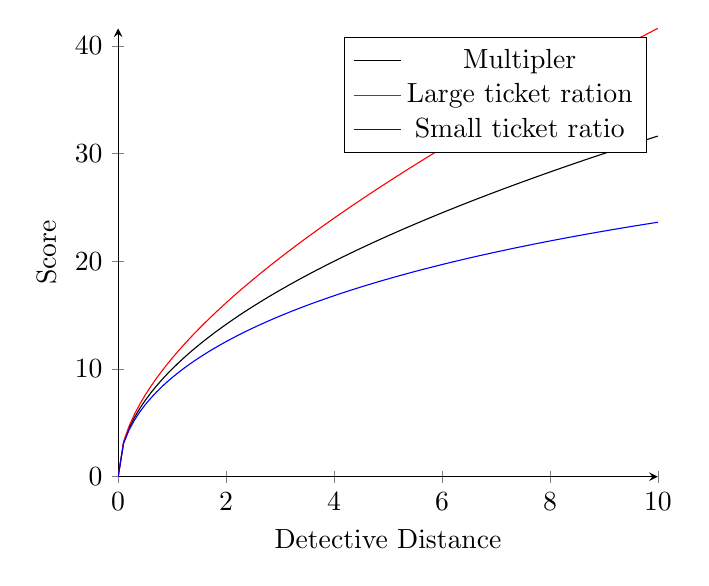
\begin{tikzpicture}
\begin{axis}[
    axis lines = left,
    xlabel = {Detective Distance},
    ylabel = {Score},
]
%Below the red parabola is defined
\addplot [
    domain=0:10, 
    samples=100, 
    color=black,
]
{(1-1)*x + (1-1)*x + 10*x^0.5};
\addlegendentry{Multipler}
%Below the red parabola is defined
\addplot [
    domain=0:10, 
    samples=100, 
    color=red,
]
{(2-1)*x + (1-1)*x + 10*x^0.5};
\addlegendentry{Large ticket ration}
%Here the blue parabloa is defined
\addplot [
    domain=0:10, 
    samples=100, 
    color=blue,
    ]
    {(0.2-1)*x + (1-1)*x + 10*x^0.5};
\addlegendentry{Small ticket ratio}
 
\end{axis}
\end{tikzpicture}
\end{figure}
\subsection{Pruning}
To avoid extra work we prune branches that have become unnecessary each time the game advances. We achieve this by setting the root of the tree to be the node containing the last played move, thus making unneeded nodes unreachable. When pruning we pause the game tree and restart it on the previous depth once pruning is completed, this helps us to avoid any concurrency issues. The results of the pruning extends our search depth a few levels after which it reaches an equilibrium between the moves being pruned and the expanding search tree.
\begin{figure}[h!]
  \centering
  	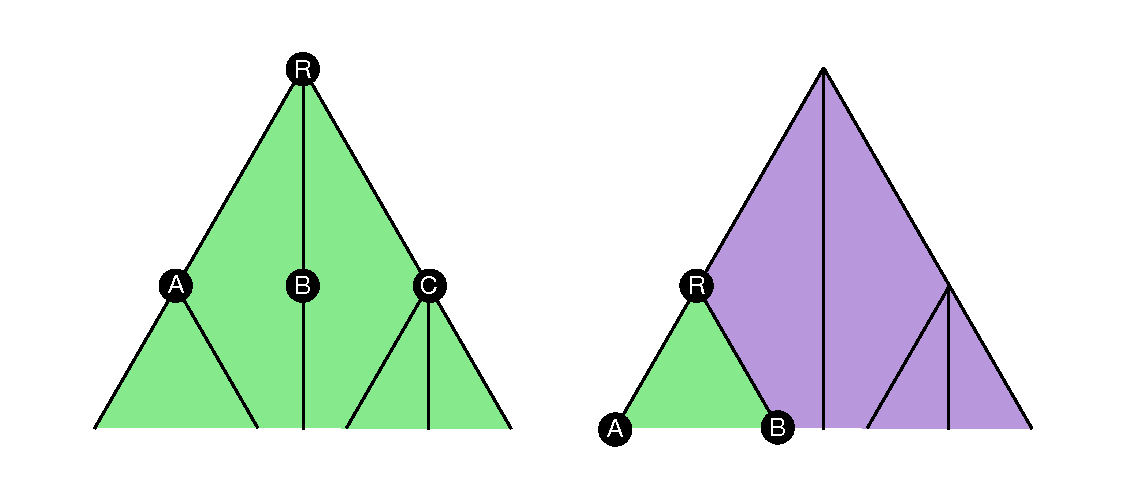
\includegraphics[width = 15cm]{TreePruning}\\
  \caption{After making move A, we can prune all other moves and their subsequent moves.}
\end{figure}
\section{Threading}

\begin{Parellelisation}
\centering
  \begin{subfigure}[b]{0.48\textwidth}
    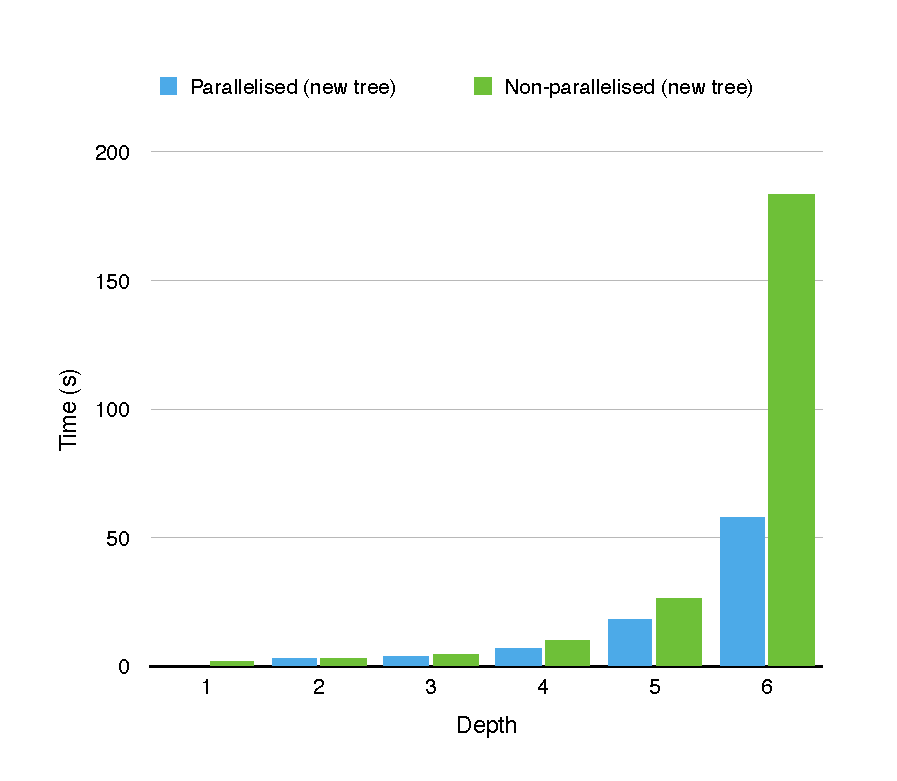
\includegraphics[width=\textwidth]{graph1}
    \caption{First iteration of the game tree}
    \label{fig:1}
  \end{subfigure}
  %
  \begin{subfigure}[b]{0.48\textwidth}
    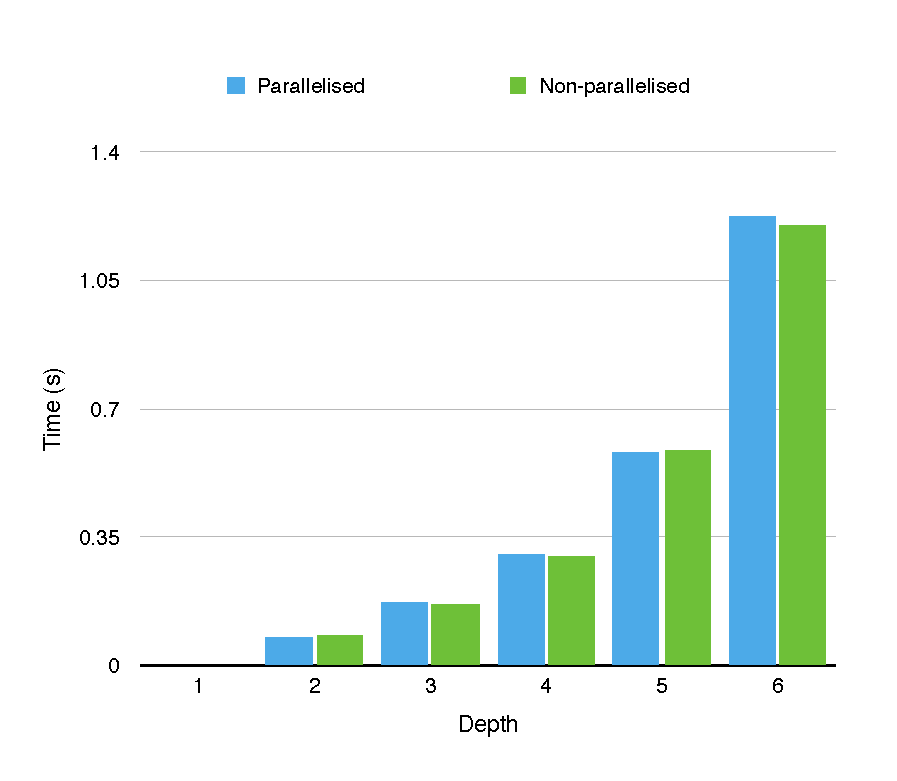
\includegraphics[width=\textwidth]{graph2}
    \caption{Subsequent iterations of the game tree}
    \label{fig:2}
  \end{subfigure}
\end{figure}

\section{Results}
The AI we have produced has very promising results and does make smart moves. However, we are still commonly coming up against errors which we believe are a result of threading issues. This means that they are very difficult to debug and in retrospect we believe that given the short amount of time provided, it would have been wise to keep our tree simple and focus on reaching to greater search depths. This would mean that we could consider moves further ahead, something that is the hallmark of a good player.\\
\\
The graphs above highlight the efficiency of using parallelisation in our alpha-beta algorithm. When running the tree from ??? we consistently get better results when using parallelisation, particularly in higher depth searches where we are getting a ~3x speed increase. When running subsequent iterations the two approaches are roughly equal, erring slightly on the slower side for the parallelised approach which makes sense given that we are starting new threads. We would expect the second graph to be equal as we are caching our tree and These graphs also highlight the time difference in reusing our game tree.
\end{document}










